\documentclass[12pt]{article}
\usepackage[english]{babel}
\usepackage[utf8x]{inputenc}
\usepackage{amsmath}
\usepackage{graphicx}
\usepackage{subcaption}
\usepackage[export]{adjustbox}
\graphicspath{ {./images/} }
\usepackage{hyperref}
\hypersetup{
    colorlinks=true,
    linkcolor=blue,
    filecolor=magenta,      
    urlcolor=blue,
}
 
\usepackage[colorinlistoftodos]{todonotes}

\begin{document}

\begin{titlepage}

\newcommand{\HRule}{\rule{\linewidth}{0.5mm}} 

\center
-------------------------------------------------------------------------------------

\textsc{\LARGE Politenico di Milano}\\[1cm]
\textsc{\Large Dipartimento Elettronica, Informazione e Bioingegneria}\\[0.5cm] 
\textsc{\large Embdedded Systems Project}\\[0.5cm] 

%----------------------------------------------------------------------------------------
%	TITLE SECTION
%----------------------------------------------------------------------------------------

\HRule \\[0.4cm]
{ \huge \bfseries Square Root For bfloat16}\\[0.4cm]
\HRule \\[1.5cm]
 
%----------------------------------------------------------------------------------------
%	AUTHOR SECTION
%----------------------------------------------------------------------------------------

\begin{minipage}{0.4\textwidth}
\begin{flushleft} \large
\emph{Authors:}\\
Francesco \textsc{Monti} \\
Fabio \textsc{Nappi} \\
Davide \textsc{Piovani} 
\end{flushleft}
\end{minipage}
~
\begin{minipage}{0.4\textwidth}
\begin{flushright} \large
\emph{Supervisor:} \\
Dr. Davide \textsc{Zoni}
\end{flushright}
\end{minipage}\\[1.5cm]


%----------------------------------------------------------------------------------------
%	DATE SECTION
%----------------------------------------------------------------------------------------

{\large \today}\\[2cm] 

%----------------------------------------------------------------------------------------
%	LOGO SECTION
%----------------------------------------------------------------------------------------

\begin{figure}[h]
\begin{subfigure}{0.5\textwidth}

\includegraphics[width=150pt, left]{Logo_Politecnico_Milano.png}
\end{subfigure} 
\begin{subfigure}{0.5\textwidth}

\includegraphics[width=100pt, right]{heaplogo.pdf}
\end{subfigure}
\end{figure} 
 
%----------------------------------------------------------------------------------------

\vfill

\end{titlepage}


\begin{abstract}
Your abstract. - Summarize your work.
\end{abstract}

\section{Introduction}
In order to represent real numbers in computer memory, a common approach is to use a floating point format. Depending on the type of encoding used, those formats occupy different memory sizes, usually 32-bits (Single precision floating point, or binary32) or 64-bits (Double precision floating point, or binary64). \\
The value F given by the floating point format, of any kind, can be expressed as:
$$F = (-1)^{S}*M*2^{E} $$
\\
Where 
\begin{itemize}
\item S is the sign (0 for positive, 1 for negative)
\item E is the exponent
\item M is the Mantissa (also called Significand)
\end{itemize}
Floating-point formats and arithmetic operations are specified by the IEEE 754 standard. \\
Under this standard (n is the number of bits reserved to the exponent):
\begin{itemize}
\item The exponent E is unsigned, with values between 0 and ($2^{n} -1$)
\item	The exponent E is biased, meaning that is encoded using an offset-binary representation, with the zero offset being $2^{n-1} – 1$
\item	The mantissa has an hidden bit, always set to 1; therefore, the actual mantissa is 1.M
\item	The standard also introduces some special values, for different purposes, such as Infinite and Not-a-Number
\end{itemize}

The single and double precision floating point representations are the two most used in modern computers and mobile phones. These devices usually aren’t particularly constrained by memory space and may actually need the accuracy offered by a 32-bit or even 64-bit representation.\\
On the other hand, many Embedded Systems are memory and power constrained, and don’t need that much accuracy in order to perform their tasks. So, they may implement the half-precision floating-point format, also called binary16. \\
This standard requires 1 bit for the sign, 5 bits for the exponent and 10 bits for the mantissa. \\
However, another standard has been recently developed, the bfloat16 (Brain Floating Point) floating-point format. This standard requires 1 bit for the sign, 8 bits for the exponent and 7 for the mantissa. \\
This format is a truncated version of the binary32 with the intent of accelerating machine learning and near-sensor computing. It preserves the approximate dynamic range of 32-bit floating-point numbers by retaining 8 exponent bits, but supports only an 8-bit precision rather than the 24-bit significand of the binary32 format. 

\begin{figure}[h]
\centering
\captionsetup{justification=centering}
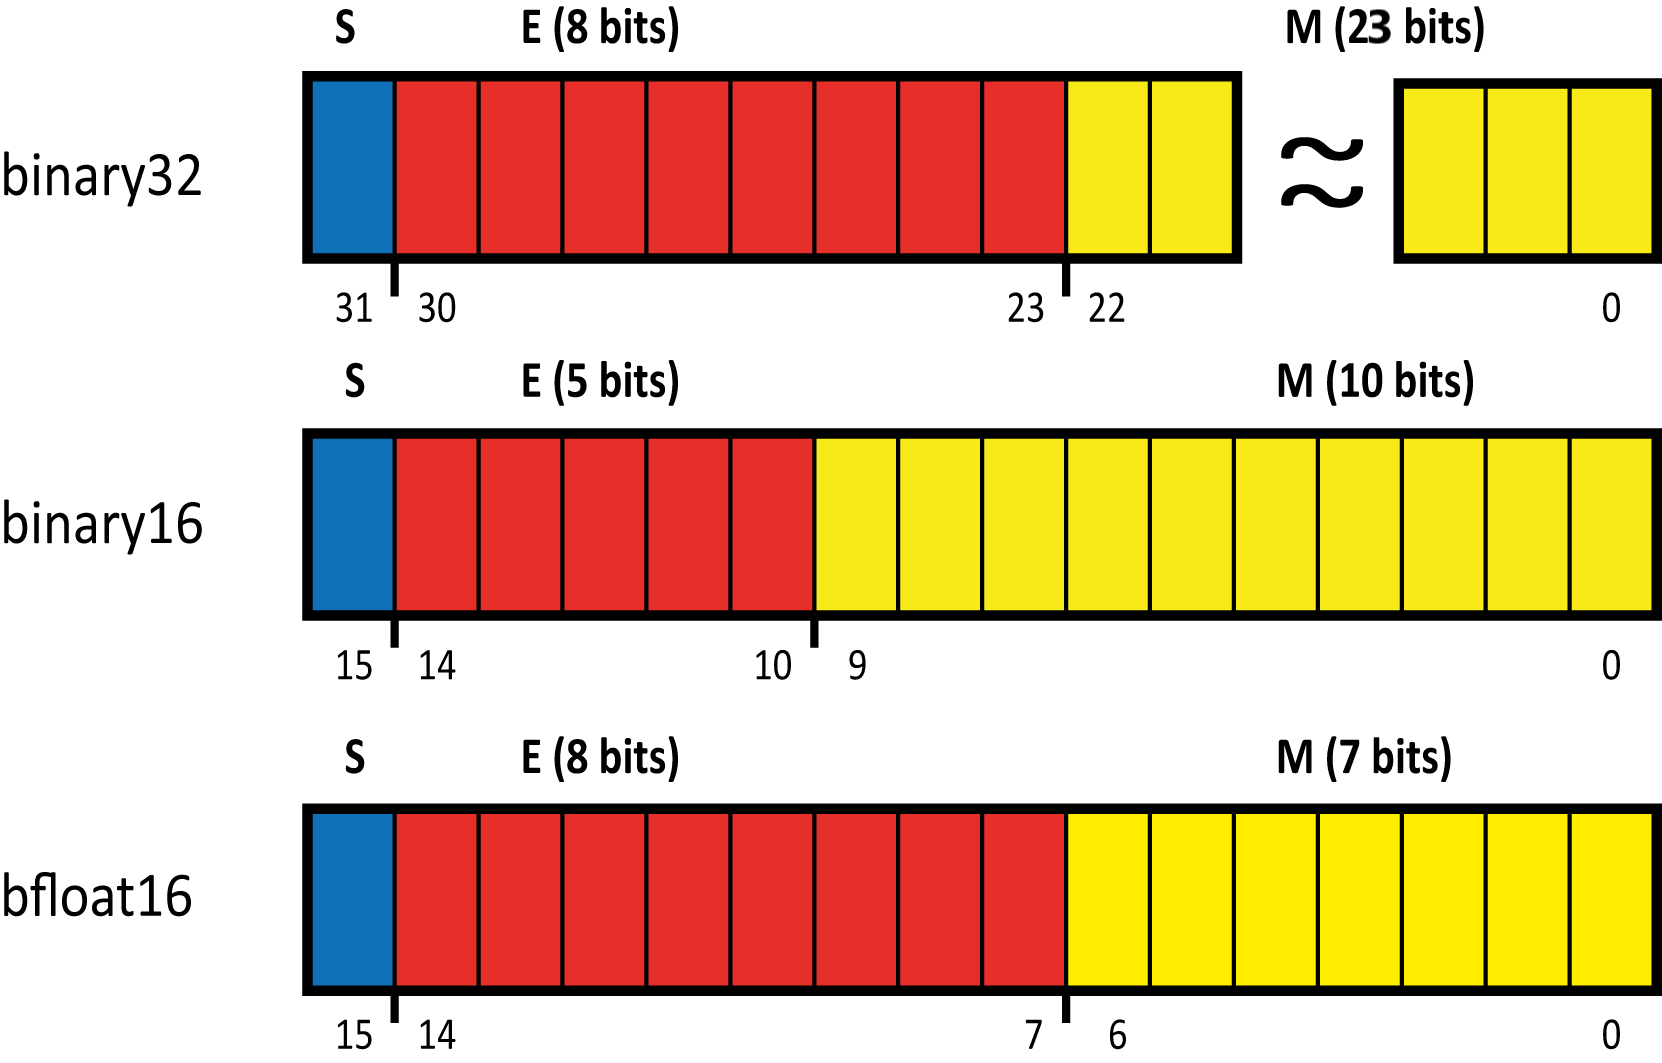
\includegraphics{float.png}	
\caption{How the bits are assigned in the different standards. \\From top to bottom: binary32, binary16, bfloat16}
\end{figure}

Heap Lab has already developed an open source FPU (\url{https://gitlab.com/davide.zoni/bfloat_fpu_systemverilog}) supporting the most common operations for bfloat16 operands. Therefore, the goals of our project is:
\begin{itemize}
\item Add support for Square Root operation
\item Verify the implementation correctness, comparing the results produced by our design with the ones obtained from the C function sqrt
\item Add support for the INVSQRT operation
\end{itemize}

\section{Design and Implementation}

\section{Experimental Results}

\section{Conclusions}

\end{document}
